\subsubsection{Analysis of Hemisphere Structure}
Next, to establish how AFM measures the topography and nanomechanics of simple geometries, we probed imaging of elastic hemispheres. Simulations focused on the perceived compression of the structure's central scanline. The spherical/cylindrical structures model the two-dimensional compression of DNA imaging along the transverse axis\cite{sotres2010afm,li2014atomic}. The hemisphere is modelled as a three-dimensional elastic part in ABAQUS with a fixed, rigid base beneath. Unlike the indentation of a full sphere with a single contact point at the base, the fixed base of a hemisphere alleviates the compression of the surface. This produces less ambiguity as the elastic response follows the Hertzian model and negates the consideration of typical double contact required for a full sphere. 

As illustrated in Figure\ref{fig: Hemisphere Compression Plot}A, except when indenting the very centre of the hemisphere, the AFM tip will first contact the hemisphere laterally such that the experienced force and tip coordinates are offset. Consequently, this effect broadens the apparent surface depending on the hard-sphere/ tangential contact. Shown in Figure \ref{fig: Hemisphere Compression Plot}B, C are results for a sharp and blunt tip, respectively. The figures show heat maps of the indentation force across the cross-section of the scan line. Subsequently, the AFM appearance for a given reference force is produced from the corresponding contour of equal force, fitted using a smooth 2D cubic spline. 
%The indentation force at each position is mapped to the 2D grid of the scan domain.

As is common in nanomechanical analysis by AFM \cite{sun2021determination,DIMITRIADIS20022798,kontomaris2019determination}, we quantify the surface stiffness by fitting the force-indentation curves, clipped to equal depths, by Hertz model (Equation \ref{eq: Hertz}). This yields an effective Youngs modulus, $\frac{E_{AFM}}{E_{Sample}}$, as a function of relative lateral position, $x/R$, shown in Figure \ref{fig: Hemisphere Compression Plot}D. Due to the geometry, the indentation of the centre has the greatest contact radius and surface extent below; consequently, the elastic response is more significant. Conversely, indentations along the sides of the hemisphere are softer due to a smaller contact radius and uneven tangential force. Moreover, as the indentation force varies as a function of the contact radius, the variation in Young's modulus over the scan position emulates the same broadening as in the apparent topography. Larger indenters produce a flatter fitted Young's modulus highlighting that a greater effective stiffness is experienced at larger indenter-surface ratios.

However, as shown in Figure \ref{fig: Hemisphere Compression Plot}E, these effects depend on the depth of surface indentation. Fitting indentation data clipped to given depths produces the effective Young's modulus for the corresponding indentation force. As force/ depth increases, the measured Young's modulus approximates the sample's value more closely. At the centre, all indenters converge on an overfit value; conversely, the softened response along the edge is further highlighted in under-fitted values.
%Indenter sizes produce little variation beyond changing the force range.

To quantify the lateral resolution/ apparent width of the hemisphere for varying imaging force, we analyse the Full Width Half Maxima(FWHM)\cite{sotres2010afm}. FWHM is calculated from the roots of the contour splines at half the maximum value. Figure \ref{fig: Hemisphere Compression Plot}F shows FWHM decreases asymptotically as the indentation force decreases. As the force increases, the sample is indented to greater depth producing tighter, compressed force contours and narrowing the surface's appearance. As noted in similar experimental work on spherical nanoparticles by Junno \textit{et al.}\cite{junno1995controlled}, as AFM images are convolutions of the samples and tip geometries, FWHM is not directly indicative of image accuracy, and an overestimated is expected. 
%The nonlinear behaviour of the FWHM highlights that the compression producing the force contours is not a simple linear relationship.

\begin{figure}[htp]
    \centering
    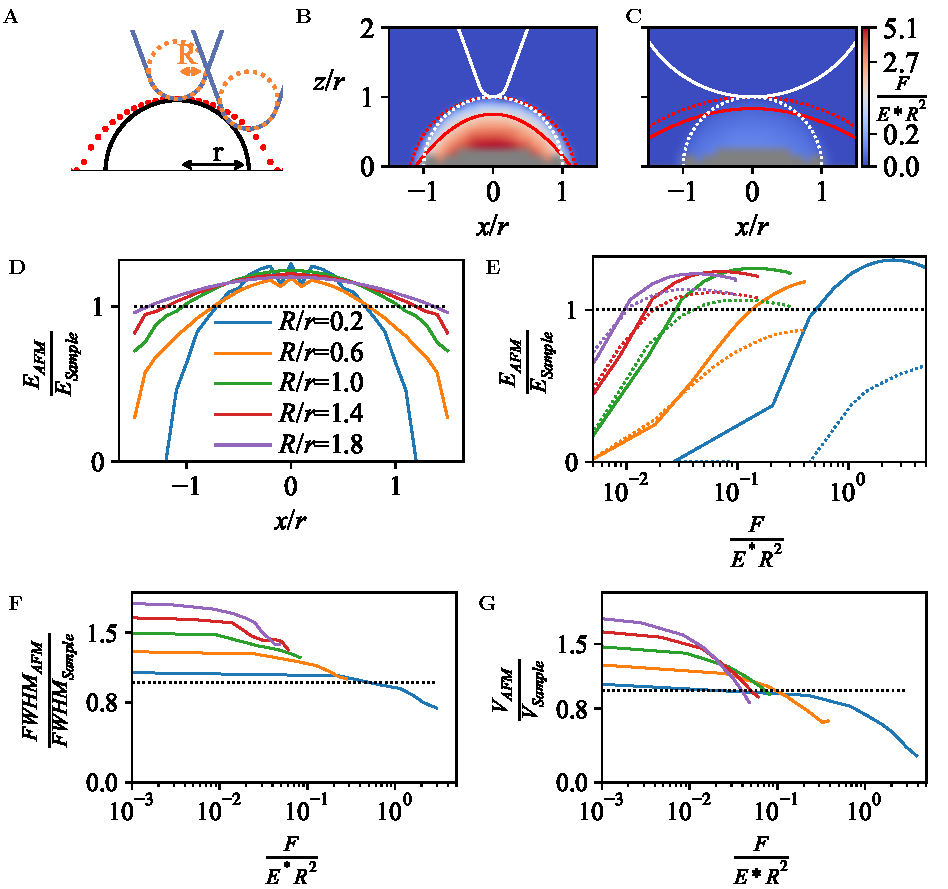
\includegraphics[width=\linewidth]{Figures/Figure3.pdf} 
    \caption{\label{fig: Hemisphere Compression Plot}(A) Geometry of scan along the central axis of a hemisphere. Three-dimensional geometry is produced by rotating the indenter and semi-circle around the central z-axis. The hemisphere is shown in black with a radius $r$. Indenter geometry is shown in blue, with the circular tip of radius $R$ in orange. Red points indicate initial scan positions (Hard sphere contact points). (B) Interpolated two-dimensional heat map of indentation force over the scanning axis for hemisphere structure with indenter $R/r=0.2$. Including overlayed contour of constant force, $\frac{F}{E^*R^2} = 0.227 $, shown in solid red. The indenter is solid white, and the surface is dotted white. Points of zero force/ hard sphere contact are shown in dotted red. A mask excludes positions with no indentation data shown in grey. (C) Interpolated two-dimensional heat map of indentation force over the scanning axis for hemisphere structure with indenter $R/r=1.4$. Including overlayed contour of constant force, $\frac{F}{E^*R^2} = 0.227 $, shown in solid red. The indenter is solid white, and the surface is dotted white. Points of zero force/ hard sphere contact are shown in dotted red. A mask excludes positions with no indentation data shown in grey. (D) Apparent Young's modulus measured across scan positions for each indenter radius ($R/r$). (E) Apparent Young's modulus variation over contour force for each indenter radius($R/r$). Measured at the centre (solid line) and at the surface edge (dashed). (F) Relative FWHM of the contour divided by FWHM of true geometry ($FWHM^*=\frac{FWHM_{AFM}}{FWHM_{Sample}}$) variation over contour force for each indenter radius($R/r$). (G)  Volume variation over contour force in spherical structures for each indenter radius($R/r$).}
\end{figure}

A similar analysis of the measured volume shows that the tip convolution overestimated the hemisphere volume. Volume is calculated using discrete, numerical integrals of contour splines. As the indentation force increases, more significant compression reduces the apparent appearance. As indenter size decreases, larger forces are required to achieve the same relative decrease in volume. This is expected as smaller indenters have smaller contact areas and complement experimental volumetric measurements of protein complexes with AFM\cite{wu2008analysis,fuentes2013afm}. 

Overall, the data illustrate how strongly the measured topography and nanomechanics may depend on tip and sample geometry and the applied forces in an AFM experiment. Analysis of the compression displayed that increasing the indenter-to-surface ratio results in lower indentation forces. As the surface-indenter ratio/contact radius increases, the forces are spread over a larger area, resulting in less deformation for the same force.